Om meer over je systeem te weten te komen is er de System Information\index{system information} (Systeeminformatie\index{systeeminformatie} applicatie. System Information geeft je heel veel informatie over je Windows systeem en de hardware waarop het draait. Het geeft je inzicht in de hardware, software en systeemonderdelen. Het kan helpen bij het zoeken naar problemen met hardware en drivers.

Om System Information te openen:
\begin{itemize}
\item Klik op het zoek icoon en zoek op System Information
\item Gebruik Windows-Toets + R en run msinfo32\index{msinfo32}
\end{itemize}

\begin{minipage}[t]{\linewidth}
\raggedright
\adjustbox{valign=t}{%
	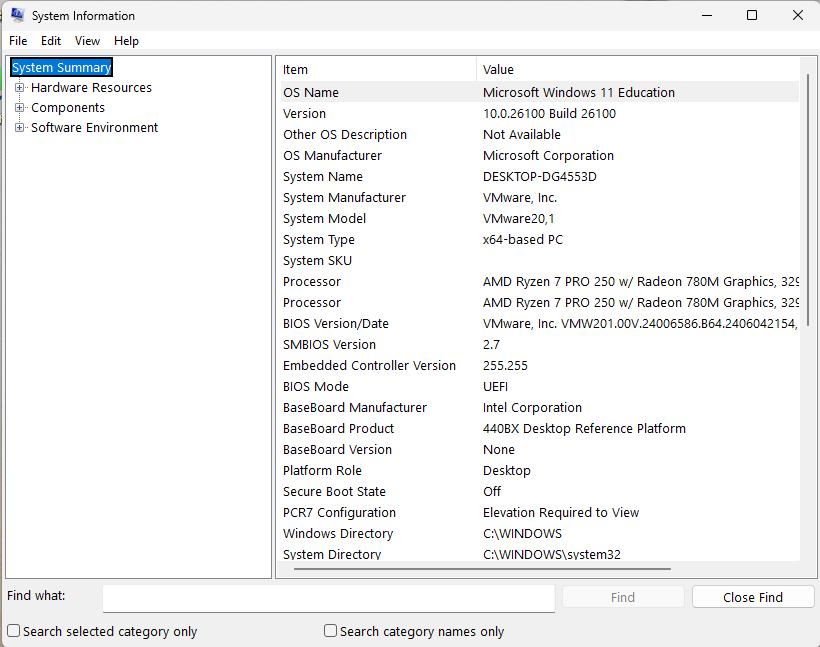
\includegraphics[width=0.99\linewidth]{sysinfo.png}%
}
\end{minipage}

